%preamble
\documentclass[letterpaper]{article}
\synctex=1
\usepackage{graphicx}
\graphicspath{ {images/} }

\usepackage{lipsum}
\usepackage{float}
% \bibliographystyle{IEEEtran}
\bibliographystyle{ieeetr}
%actual document
\begin{document}

  % \maketitle %insert titlepage here
  \begin{titlepage}
    \begin{center}
        \vspace*{1cm}
        \Huge
        Experiment 1
        \vspace{1cm}

        Electrostatic Potentials and Fields
        \vspace{1cm}

        By: Arun Woosaree
        \vspace{1cm}

        Lab partners:
        \vspace{.25cm}
        \Large

        Fatemeh Ghafari Far

        Yvonne Hong
        \vspace{1cm}

        \Huge
        PHYS 230 Lab EH71
        \vspace{1cm}

        TA: Andrei Tetriakov
        \vspace{1cm}

        Date of Lab: \today
        \vfill
    \end{center}
\end{titlepage}

\section{Introduction}
% Begin with experiment’s objectives\\
% Give physical background:\\
% ○ Describe investigated/used\\
% phenomena e.g. Gauss’s law,\\
% field lines, equipotential lines.\\
% ○ Do not copy text from a
% textbook/manual\\
% Provide equations you used\\
% ○ Identify all symbols\\

In this experiment, we explore Gauss's Law using a circular capacitor, and
we map electric potential and the electric field of a parallel plate capacitor.
A capacitor is essentially two charged conductors separated by some insulator.
We can measure the potential differences in the region between the charged conductors,
and since our geometry is simple, the electric potential can be compared with
predictions made using Gauss's Law. We can use a contour map consisting of equipotential
curves, which can then be used to construct the corresponding electric field lines.
By analyzing field patterns, we can determine the charge distribution on the surface of
the charged conductors.

The electric field \textbf{E} is defined such that a positive test charge $q$
placed in the electric field will experience a force $\textbf{F}=q\textbf{E}$.
Additionally, a certain amount of work $W=F \Delta s=qE\Delta s$ is done to move the charge
a distance $\Delta s$, parallel to the electrostatic force. The electrostatic force is
conservative, so the potential energy $U$ must decrease by $\Delta U=-qE\Delta s$.
$V$, the electric potential is defined to be potential energy per unit charge $V=U/q$.
The magnitude of an electric field at a point can be related to $V$ by
\begin{equation}
  E=-\frac{\Delta V}{\Delta s} \label{eq1}
\end{equation}

Using Gauss's law, in part 1 of the experiment we imagine a Gaussian cylinder enclosing
the inner and outer conductors of a circular capacitor. This cylinder has a radius $r$ and
length $L$ with flat end caps. Since \textbf{E} is parallel to the end caps, the flux, denoted $\Phi$ on
the end caps are zero, which leaves the curved surface of the cylinder, with area $2\pi rL$.
Since \textbf{E} is constant and perpendicular to the curved surface, the total flux $\Phi_E$ can be found
\begin{equation}
  \Phi_E = \Phi_{end1} + \Phi_cylinder + \Phi_{end2} = 0+E(2\pi rL) + 0 =\frac{Q}{\epsilon_0}
\end{equation}
\begin{figure}[H]
    \centering
    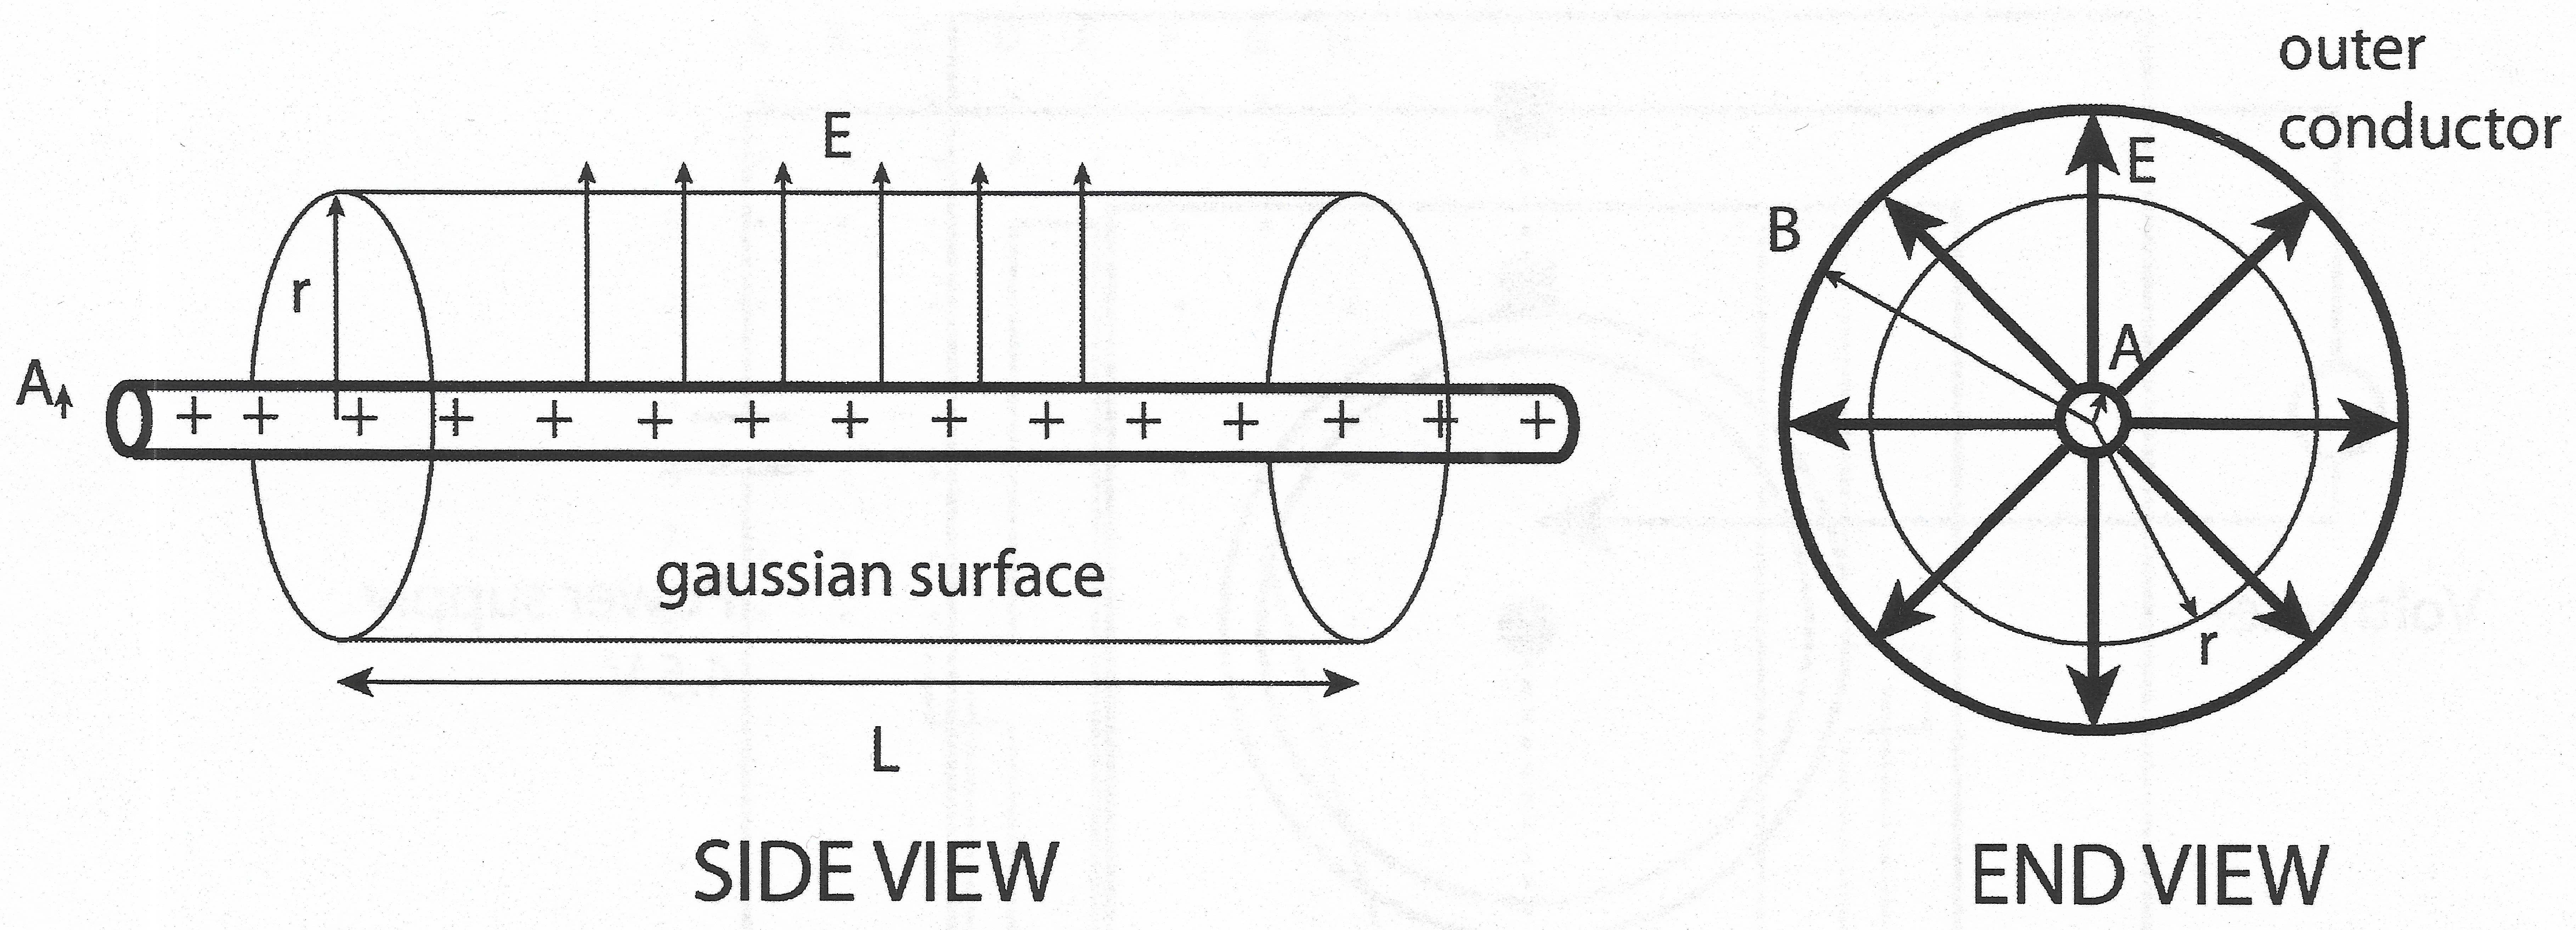
\includegraphics[width=\textwidth]{fig1.jpg}
    \caption{Gaussian Surface between two circular conductors. \cite{labmanual}}
\end{figure}

$\sigma$ is defined as the charge per unit area on the surface of the inner conductor.
The enclosed charge $Q$ enclosed by the Gaussian cylinder is $Q=(2 \pi AL)\sigma$, where
$A$ is the radius of the inner conductor, and $\epsilon_0=8.85418782 \times 10^{-12} m^{-3} kg^{-1} s^{4} A^{2}$ is the permittivity of free space.
Given the above information, the magnitude of the electric field at some radius $r$
can then be computed

\begin{equation}
  E=\frac{\sigma A}{\epsilon_0 r}
\end{equation}

If we put a probe at radius $r$, and the outer conductor has a radius $B$ then the voltage
difference between the probe and the outer conductor is
\begin{equation}
  V_r-V_B=\frac{\sigma A}{\epsilon_0 r} \ln{\frac{B}{r}}
\end{equation}
From which we can obtain the following equation if we set the voltage difference between the two conductors to have a value $V_0$
\begin{equation}
  \frac{V_r-V_B}{V_0}=\frac{\ln{\frac{B}{r}}}{\ln{\frac{B}{A}}}
\end{equation}
or alternatively,
\begin{equation}
  \ln{r} =\ln{\frac{A}{B}}(\frac{V_r-V_B}{V_0}) + ln{B}
\end{equation}
In part 2 of the experiment, we map the electric field of a parallel plate capacitor, and draw equipotential lines
which correspond to electric field lines.


\section{Experimental Method}
% List all equipment used\\
% ○ Provide parameters as detailed as
% possible: masses, frequencies,
% etc.\\
% Report what YOU DID to achieve
% experimental goals:\\
% ○ Do not use imperative clause\\
% ○ Use first person narrative or
% passive voice\\
% Based on this section you should be
% able to reproduce your results without a
% manual

\textbf{List of Equipment:}
\begin{itemize}
  \item Circular capacitor (Figure 2)
  \item Parallel plate capacitor (Figure 3)
  \item Power Supply
  \item Voltmeter
\end{itemize}
For both parts of the experiment, the power supply was set to 4.5V. \\This is $V_0$ in equations 5 and 6.
\newpage
\subsection{Part 1}
In Part 1 of the experiment, a circuit was constructed using the above materials, as shown in the Figure 2 below.
The positive lead of the power supply was connected to the center of the circular capacitor, and the negative lead
was connected to the negative end on the voltmeter, and a probe was attached to the positive end of the voltmeter.
The probe was then touched at various radii on the circular capacitor, and the measured voltages were recorded in
a spreadsheet. The data was then plotted as the natural log of radius $r$ versus the voltage difference at radius $r$
to produce a linear graph. (Figure 4) The inner radius $A$ and outer radius $B$ as seen in Figure 1 were measured in centimetres, with a ruler
that had millimetre markings.
\begin{figure}[H]
    \centering
    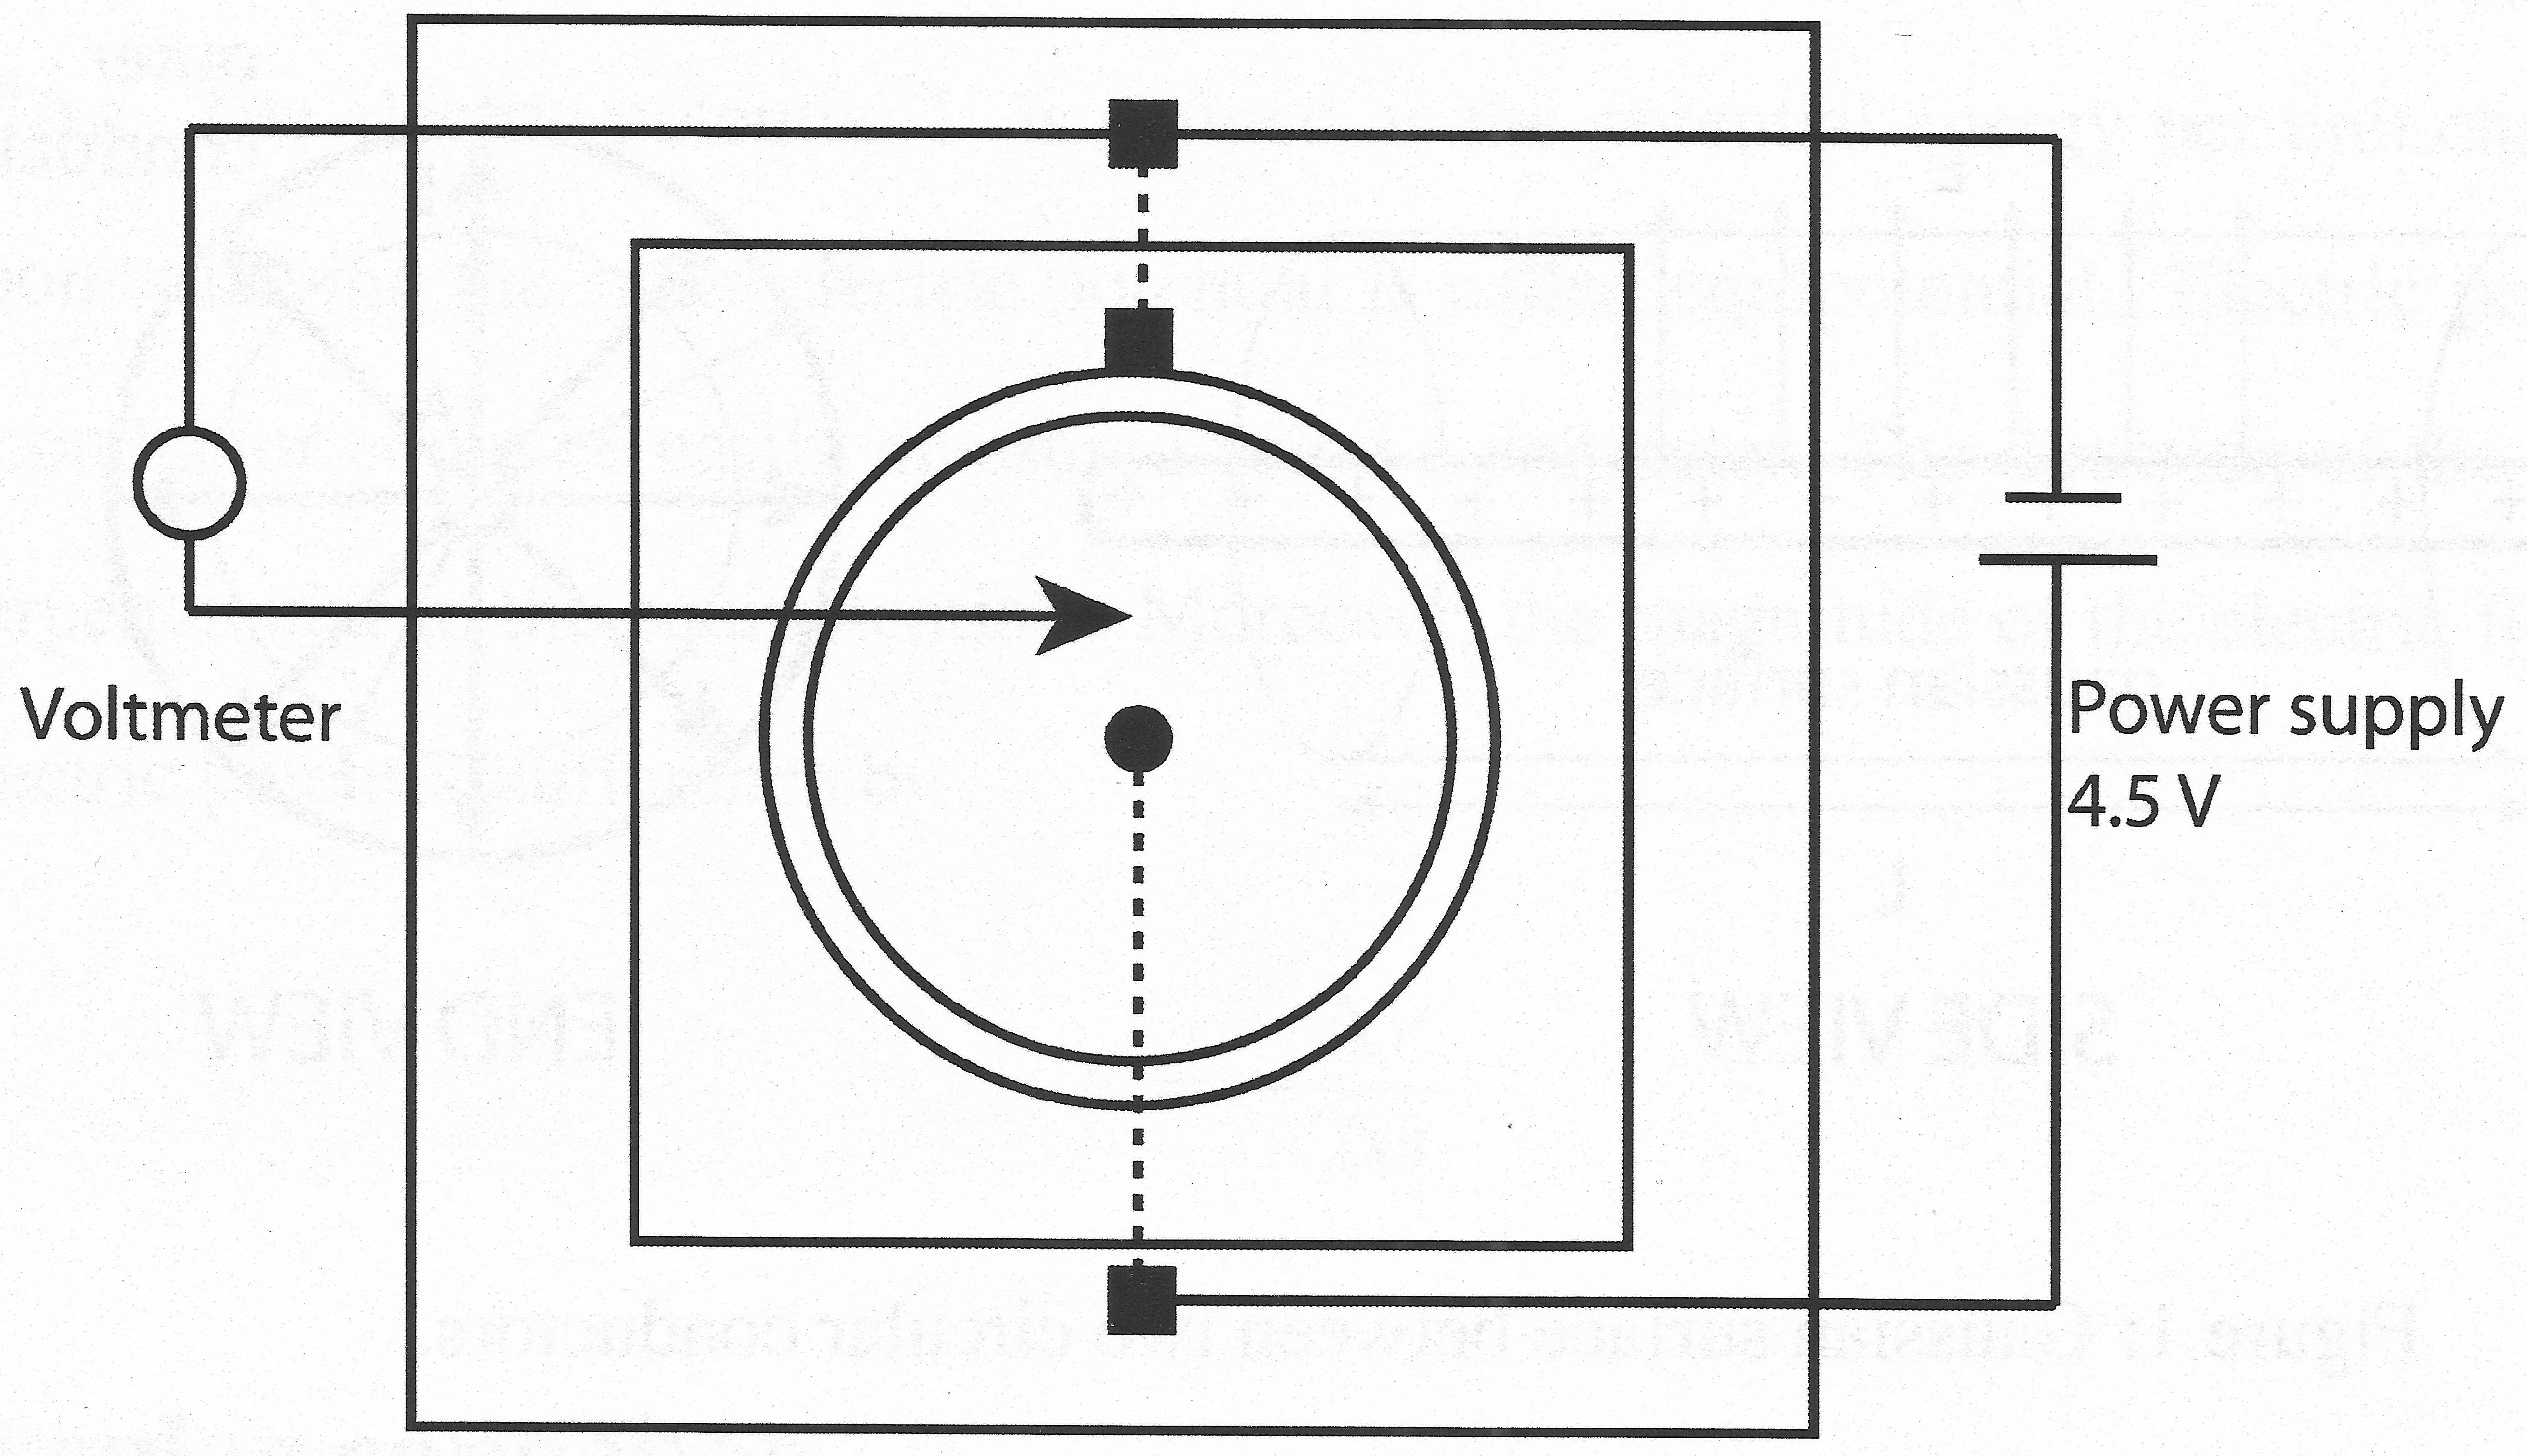
\includegraphics[width=.9\textwidth]{fig2.jpg}
    \caption{Measuring the voltage difference at various radii $r$ between two circular conductors. \cite{labmanual}}
\end{figure}


\subsection{Part 2}
In Part 2 of the experiment, a circuit was constructed using the parallel plate capacitor.
The positive end of the power supply was connected to one plate of the capacitor, and the negative
lead of the power suppply was connected to the side of the capacitor with markings for measuring potential
differences, and the negative end of the voltmeter. The probe remained connected to the positive end of the
voltmeter, as in Part 1. Once again, the probe was touched at various points on the capacitor, and the
voltage differences were recorded in a spreadsheet, from which Figures 5 and 6 were produced.

\begin{figure}[H]
  \centering
  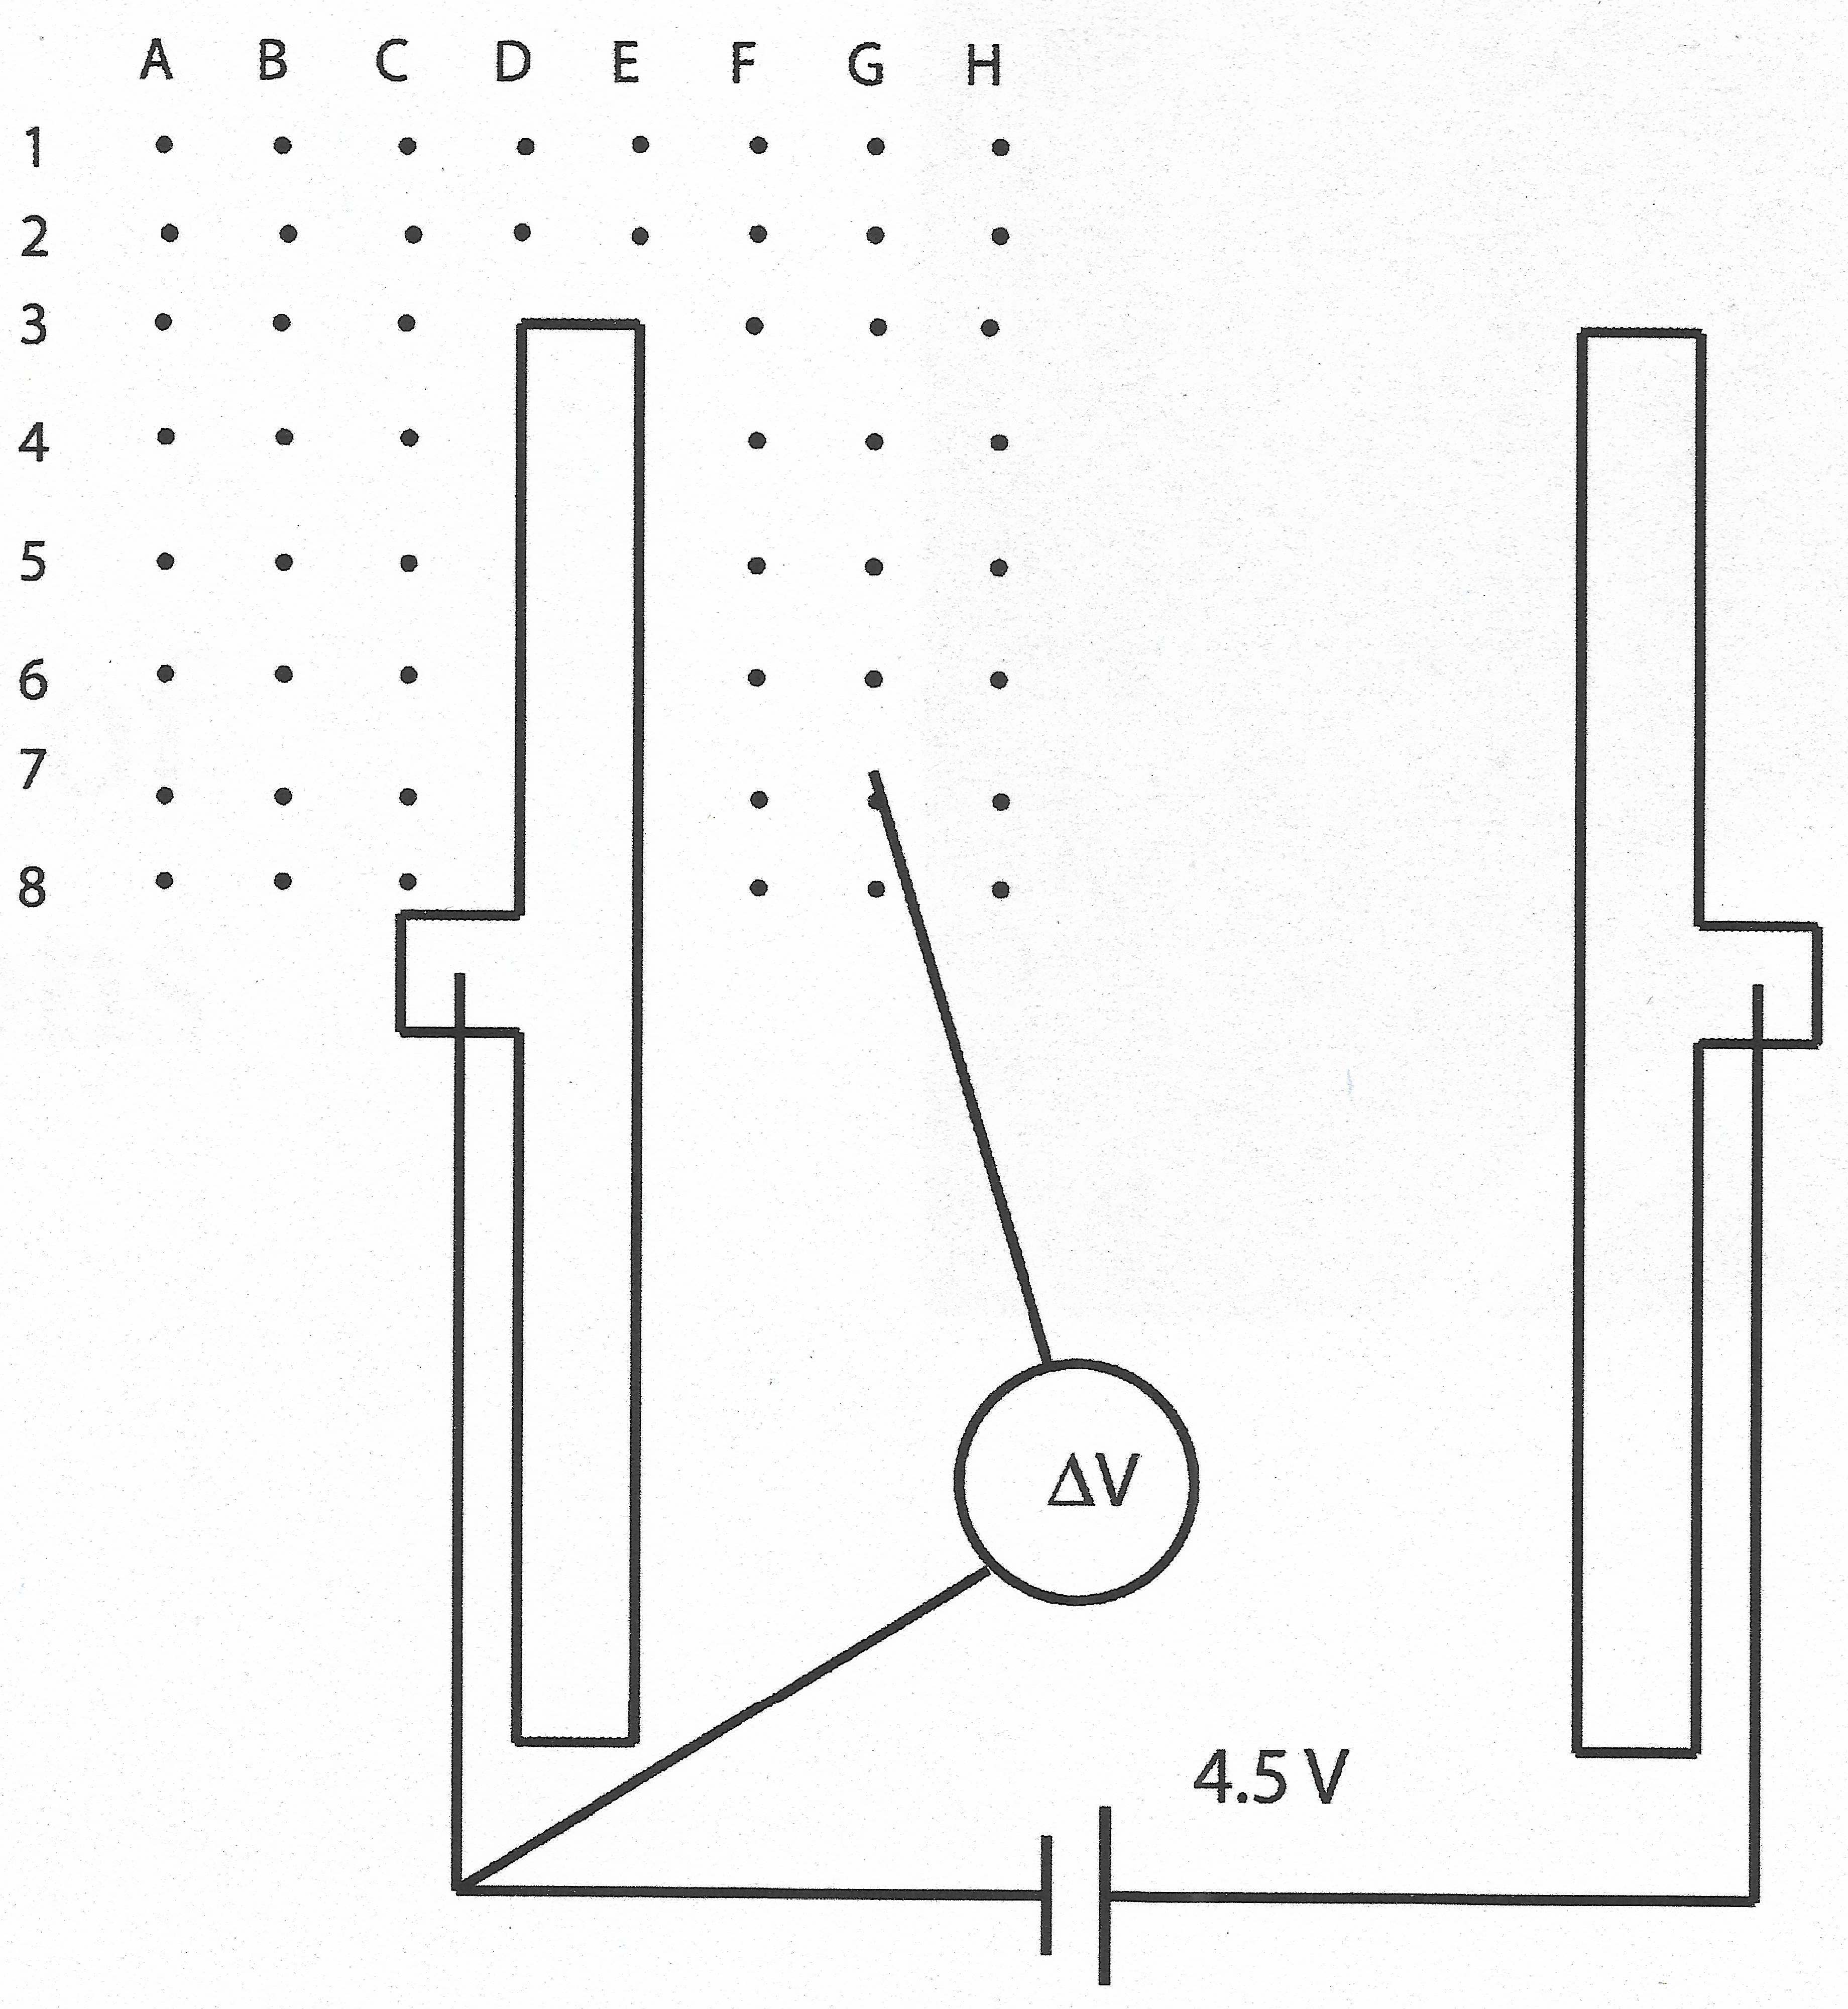
\includegraphics[width=.7\textwidth]{fig3.jpg}
  \caption{Measuring the voltage difference in a region between two parallel conductors. \cite{labmanual}}
\end{figure}

% When the apparatus illustrated above is set up, i.e. the lengths ‘r’ and ‘R’ are known, the center of the spark tape is marked when the bob is hanging freely at rest, and the bob is at the starting position, being held by the electromagnet, and the string is steadied to lessen any vibrations, the power going to the electromagnet is cut, and as a result, the bob is released from rest. The ‘RUN’ button on the spark timer is immediately (as best as humanly possible) held down, until the bob reaches approximately the maximum height on the other side of the track, or when one half of the period of the pendulum is completed.
%
% The spark timer is set to spark 30 times a second, so the time elapsed between each burn hole on the spark tape is 1/30th of a second. Once the spark tape is obtained from the apparatus, we need to measure the displacements of the glider as it was moving. To do so, we use a meter stick, and a displacement of 0.00m is taken to be the at the center of the spark tape, which is the point that was marked while the bob hangs freely at rest. This means that the initial displacement of the bob is taken to be a negative displacement, and the points after the bob passes the center are taken to be positive.
%
% After measuring the displacements of the bob, we enter the data points into Excel, and also calculate the time elapsed for each data point. (Ex. At the 10th burn hole, the time elapsed would be 10*1/30 seconds). From this data, we can calculate EK , EP , and ET  using equations  5,9 and 10 and plot them on a graph as a function of time. The ET curve was fit to a linear regression, and the EK and EP curves were fit to quadratic curves.

\section{Results}


Should be a coherent text\\
Present all data and calculations with words. Examples:\\
○ “Row data for free-fall acceleration measurements is given by Table 1.”\\
○ “In order to find the acceleration we plot doulbed distance as a function of
time squired as is shown by Figure 1.” or “To find the acceleration we
linearize Equation 1 as d(x)=ax, where x=t2/2 and plot it on Figure 1”.\\
○ “The slope of the graph corresponds to the acceleration and can be found
along with the uncertainty using LINEST(see Table 2)”\\
○ “The uncertainty in distance is calculated as d= x+ y”\\
○ “Finally, the acceleration due to gravity is 9.81± 0.03 m/s2 ”\\
All figures and should have label and caption \\(e.g. “Figure 1: position as a function
of time during free fall”).\\
Use scientific notation (103, not 1E3) and appropriate significant digits

\section{Part 1}
% Part I\\
% Linearized equation: provide
% all parameters e.g. variables,
% slope, intercept, etc.\\
% Linear graph: add trendline,
% provide fitting parameters
% (slope, intercept)\\
% Give values A and B obtained
% from the graph and measured
% directly\\
% Use Linest to find
% uncertainties\\

Raw data recorded while measuring potential differences at various radii on
the circular capacitor is given by Table 1.
\begin{table}[H]
\centering
\begin{tabular}{|c|c|}
\hline
 Radius $r$ (cm) & Voltage (V)\\ \hline
 2.5         & 3.45        \\ \hline
 3           & 3.03        \\ \hline
 3.5         & 2.63        \\ \hline
 4           & 2.27        \\ \hline
 4.5         & 1.89        \\ \hline
 5           & 1.72        \\ \hline
 5.5         & 1.49        \\ \hline
 6           & 1.26        \\ \hline
 6.5         & 0.86        \\ \hline
 7           & 0.62        \\ \hline
 7.5         & 0.59        \\ \hline
 8           & 0.45        \\ \hline
 8.5         & 0.2         \\ \hline
\end{tabular}
\caption{Raw data recorded when measuring potential differences at various radii $r$ on the circular capacitor.}
\end{table}

Using the raw data in Table 1, a linear graph is generated by taking the natural logarithm of the
radii, and setting $\ln{(r)}$ to be the y-axis. The potential difference is then divided by $V_0=4.5 V$
and plotted on the x-axis. As a result, by observing Equation 6, we can see that the
slope of the graph is $\ln{\frac{A}{B}}$, and the y-intercept is $\ln{(B)}$
\begin{figure}[H]
  \centering
  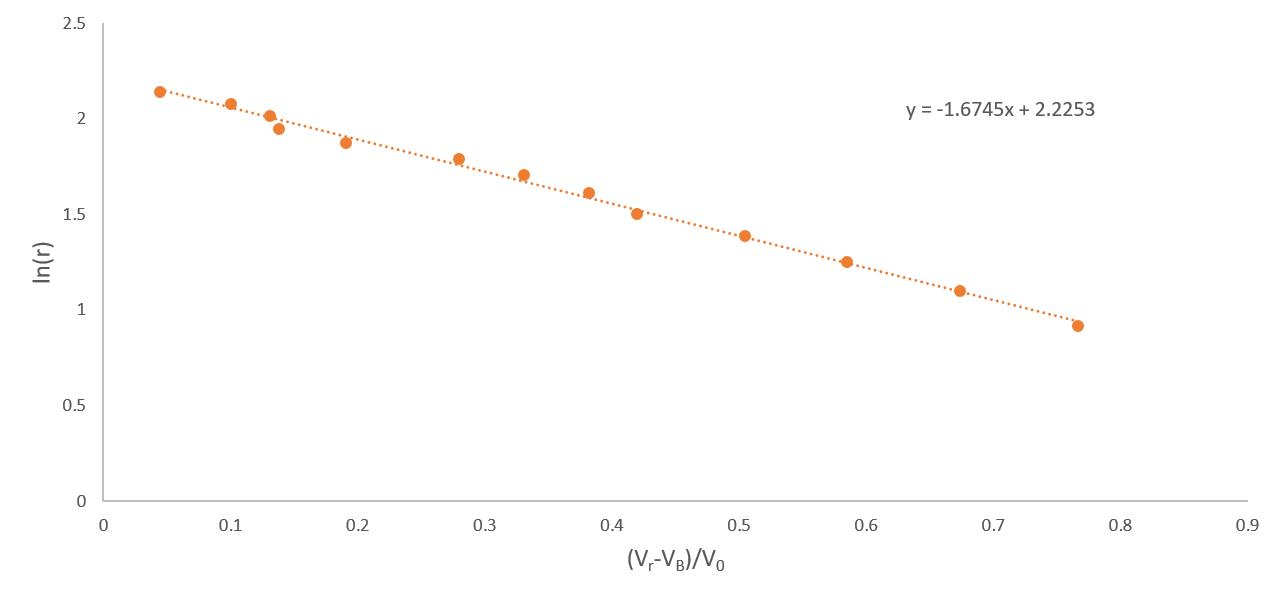
\includegraphics[width=\textwidth]{chart1.png}
  \caption{Measuring the voltage difference in a region between two parallel conductors.}
\end{figure}

\begin{table}[H]
\centering
\begin{tabular}{cc}
  Slope     & -1.674456326\pm0.03399955317 \\
  Intercept &  2.225330849\pm0.01408922355 \\
\end{tabular}
\caption{LINEST data from the graph in Figure 4}
\end{table}


From our LINEST data (Table 2), we can see that the y-intercept $\ln{(B)}=2.22533084879698$
Thus, the calculated value of $B$ from the graph can be found by exponentiating $\ln{(B)}$.\\
  $$e^{ln(B)}=B=e^{2.22533084879698}=9.25654481406370...$$
And the error can be calculated:
$$ ERROR $$
So, $B=9.3\pm NUMBER cm$ is the value for inner radius $B$ obtained from the graph.
The percent error is:
$$ \frac{|9.25654481406370-9.5|}{9.5}\times100 = 2.56\%$$
To obtain the calculated value for $A$, we see that from our LINEST data (Table 2) the slope $\ln{\frac{A}{B}}=-1.674456326$
Thus, the calculated value of $A$ can be found by
$$ e^{\ln{\frac{A}{B}}}}=e^{-1.674456326} = \frac{A}{B} = 0.1874100418... $$
$$ B \times \frac{A}{B} = A = 9.25654481406370 \times 0.1874100418 = 1.73476945...$$
So, $A=1.7\pm NUMBER cm$ is the value for outer radius $A$ obtained from the graph.
The percent error is:
$$ \frac{|1.73476945-1.9|}{1.9}\times100 = 8.70\%$$
The calculated values of $A$ and $B$ are summarized in Table 3.
\begin{table}[H]
\centering
\begin{tabular}{c|c|c|c|}
                & Measured            & Obtained from graph: & \% Error \\ \hline
Inner radius A: & 1.9 \pm 0.1 cm      & 9.3 \pm XX           &    2.56  \\ \hline
Outer radius B: & 9.5 \pm 0.1 cm      & 1.7 \pm XX           &    8.70  \\ \hline
\end{tabular}
\caption{Measured values of $A$ and $B$ compared to the calculated values obtained from the graph.}
\end{table}

\section{Part 2}
Part II\\
Provide graph from the template\\
By hand draw field lines, show charge
distribution, etc.\\
Provide the explanation, calculations,
answer questions in Discussion.\\





\begin{figure}[H]
  \centering
  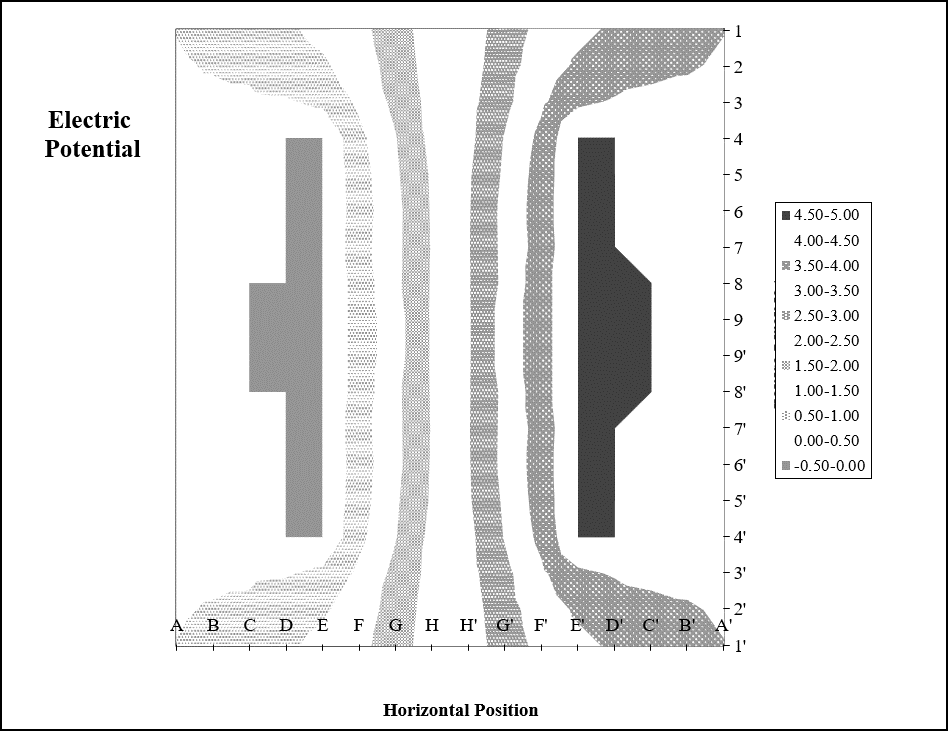
\includegraphics[width=\textwidth]{chart2.png}
  \caption{Measuring the voltage difference in a region between two parallel conductors.}
\end{figure}

\begin{figure}[H]
  \centering
  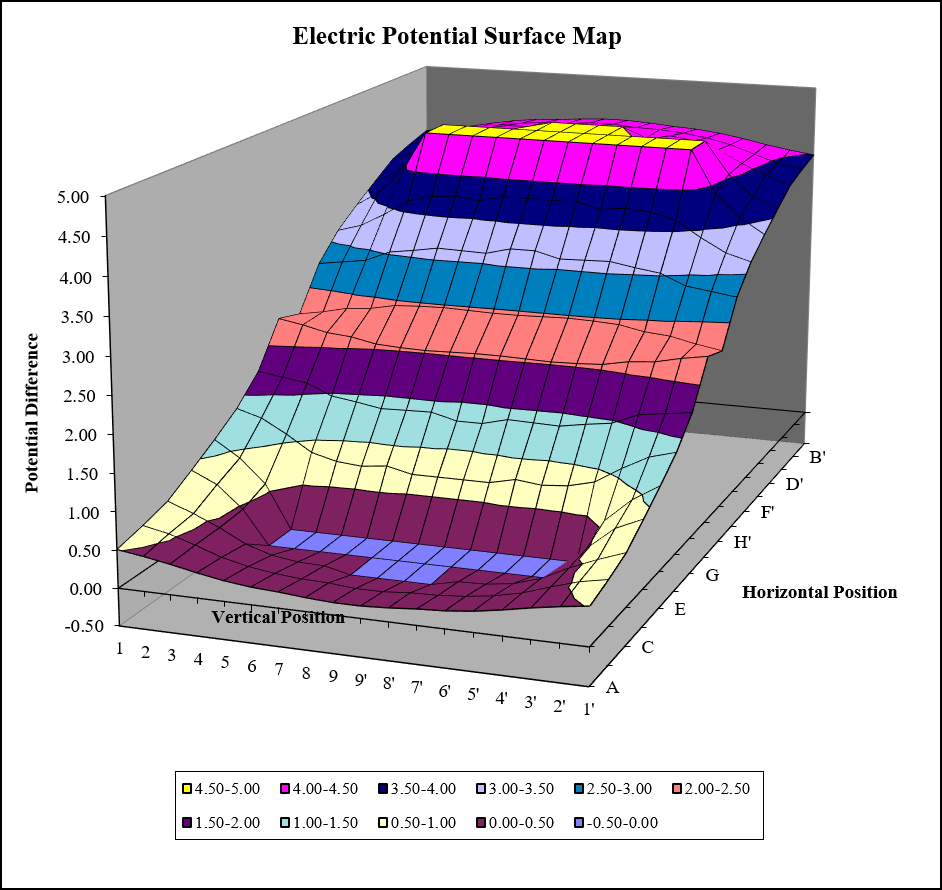
\includegraphics[width=\textwidth]{chart3.png}
  \caption{Measuring the voltage difference in a region between two parallel conductors.}
\end{figure}



\section{Discussion}
The results from the lab overall seemed reasonable, because the data fit pretty nicely to the curves that we expected them to in the graph. ET was fit to a linear curve, and EK and EP were fit to quadratic curves.  (Fig.2).  The value calculated for energy loss per second from the graph (-0.44739±0.510812 J/s) does not agree within error of the expected value we calculated (0.00161 J/s) which was calculated by measuring the initial and final displacement of the bob on the pendulum after 25 periods, finding the initial and final potential energies, calculating the total time for 25 periods, and then finding the average energy loss per second. The calculated value from the graph is 3 orders of magnitude different. However, given that the slope of the graph(fig.4) seemed almost flat, the data still seems somewhat reasonable.

We did, however have to omit 4 anomalous data points from the curve fits, because it is very unlikely that the bob was moving about 12 or 25 m/s at any point along the track. These anomalous data points can be attributed to the spark timer missing two sparks, since one missing spark would significantly impact two data points for the instantaneous velocity, since the bob would appear to move a lot faster than it actually did for two data points. It appears to move faster since the instantaneous velocity is calculated using the data points from before and after spark n, and a missing spark in the data makes it seem that the bob is moving a greater distance in a shorter time than it actually is. (see eq. 4). Two missing sparks would have caused four calculated instantaneous velocities to be significantly higher than they should be, and since instantaneous velocity is used to calculate EK on the graph, EK at the two points where the spark was missed would be significantly higher than they should be. Once can even see on the graph that the four anomalous data points are in pairs of two. (One at 20-25 J and the other at 10-15 J). Because ET includes EK, there are four anomalous data points for ET as well, at the exact same time.  Hence, these data points were ignored when fitting curves to the data.

On the graph (fig.4), we would expect to see ET as a constant, horizontal line, and indeed, the linear fit seems to be almost horizontal. The line is not horizontal, however, and it has a slight downwards slope of -0.44739±0.510812 J/s . This is due to the loss of energy. In an ideal scenario, with no energy loss, the line should be perfectly flat, however energy was being lost due to factors such as air friction, friction with the bob on the track, and vibrations on the string. At t=0, we see that ET and EK are almost the same values, as we would expect since at the beginning, the bob is not moving, so EK would be zero. (Also confirmed on the graph.) As the bob is moving down, we would expect EP to be converted into EK, and we see that on the graph, EP is decreasing as EK increases, up until EP is about 0 and EK is almost equal to ET, which is definitely observed on the graph. After that point, one would expect, and can also see on the graph that EK would be converted back into EP, until EK is almost 0, and EP is about ET. This data agrees with the law of conservation of energy, as we can visually see from the graph what types of energy are being converted, whilst observing the total energy being almost constant. (Since we are not working in an ideal scenario, and energy is lost due to factors such as friction.)

\section{Conclusions}
  In lab 8, we set up a pendulum with a 2.3kg bob hanging off of a string, and put an arced track such that the bob would be close enough to the track at any point while it swings to make a spark, with a spark timer. We then used an electromagnet to release the bob from rest, and used the spark timer to keep track of the bob’s displacements, and since the spark timer sparks at regular intervals, we had enough data to generate plots in Excel of potential energy, kinetic energy, and total energy as functions of time. The law of conservation of energy says that energy cannot be created or destroyed, but it can be converted. Theoretically, all of the Pe at the beginning should convert completely into KE, and then towards the end, all of the KE that the bob has should convert back into PE. Indeed, we do observe this behaviour in the lab, albeit not perfectly, since energy is also lost due to some of it being converted to other forms such as friction. This caused TE to decrease over time. Additionally, there were some anomalous data points that can be attributed to the spark timer missing sparks. Overall, however, the data seemed reasonable, albeit the amount of energy lost per second using the graph’s data versus taking an average after 25 periods did seem to disagree with 3 orders of magnitude.  One can observe the physics principles explored in the lab in real-life such as on a rollercoaster, where the gravitational potential energy is also converted into kinetic energy and vice versa such as when the car is going through a loop.
\bibliography{references}
\end{document}
